\chapter{Arhitektura i dizajn sustava}
		
		\iffalse
		\textbf{\textit{dio 1. revizije}}\\

		\textit{ Potrebno je opisati stil arhitekture te identificirati: podsustave, preslikavanje na radnu platformu, spremišta podataka, mrežne protokole, globalni upravljački tok i sklopovsko-programske zahtjeve. Po točkama razraditi i popratiti odgovarajućim skicama:}
	\begin{itemize}
		\item 	\textit{izbor arhitekture temeljem principa oblikovanja pokazanih na predavanjima (objasniti zašto ste baš odabrali takvu arhitekturu)}
		\item 	\textit{organizaciju sustava s najviše razine apstrakcije (npr. klijent-poslužitelj, baza podataka, datotečni sustav, grafičko sučelje)}
		\item 	\textit{organizaciju aplikacije (npr. slojevi frontend i backend, MVC arhitektura) }		
	\end{itemize}
\fi
	S najviše razine apstrakcije, arhitekturu možemo podijeliti na tri podsustava:
	\begin{itemize}
		\item Web poslužitelj
		\item Web aplikacija
		\item Baza podataka
	\end{itemize}

\vspace{15pt} 
\begin{figure}[H]
	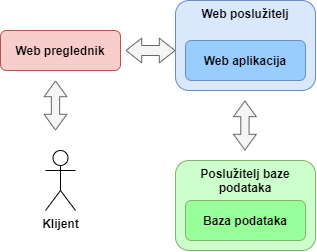
\includegraphics[scale=0.75]{slike/apstraktna-arh.PNG} %veličina slike u odnosu na originalnu datoteku i pozicija slike
	\centering
	\caption{Apstraktna arhitektura sustava}
	\label{fig:arh}
\end{figure}
\vspace{15pt}

\underline{Web preglednik} (eng. web browser) je program koji korisniku omogućuje pregled web-stranica i multimedijalnih sadržaja vezanih uz njih. Preglednik omogućuje komunikaciju između klijenta i poslužitelja. Dakle, korisnik će putem preglednika slati zahtjeve poslužitelju te će preglednik znati prikazati sadržaj koji poslužitelj vraća. \par
\vspace{10pt}
\underline{Web poslužitelj}  ima zadatak da pohranjuje, obrađuje i dostavlja klijentima web
stranice. Komunikacija između web poslužitelja i web klijenta (najčešće, web
pretraživača) odvija se korištenjem HTTP i drugih sličnih protokola (HTTPS,
HTTP/2 i različitih nadogradnji tih protokola). U komunikaciji putem HTTP-a, web
poslužitelj tipično sluša nadolazeće zahtjeve klijenata na portu 80. Web stranice koje
web poslužitelj isporučuje klijentu su HTML dokumenti, koji uključuju tekst, slike,
stilove, skripte i drugi sadržaj. \par
\vspace{10pt}
\underline{Web aplikacija} obrađuje korisnikove zahtjeve te ako je potrebno, pristupa bazi podataka i dohvaća/mijenja podatke. Nakon toga preko poslužitelja vraća korisniku odgovor u obliku HTML dokumenta koji se prikazuje u web pregledniku.\par
\vspace{10pt}
\underline{Baza podataka} pohranjuje podatke na sustavan način.  Računalni program korišten za upravljanje i ispitivanje baze podataka nazvan je sustav upravljanja bazom podataka (SUBP).\par

\vspace{15pt}
	
	Arhitektura i stil našeg sustava se može identificirati kao \textbf {višeslojni stil arhitekture}. Naime, naša arhitektura je uglavnom definirana činjenicom da koristimo \textbf{Spring Boot}. Obrazac koji se koristi u okviru radnog okvira Spring Boot je jedan od suvremenih primjera organizacije višeslojne arhitekture, a karakteriziraju ga dva principa:
	\begin{itemize}
		\item inverzija upravljanja (engl. inversion of control)
		\item ubacivanje ovisnosti (engl. dependency injection)
	\end{itemize}

	\underline{Inverzija upravljanja} funkcionira tako da korisnički napisani dijelovi (web) aplikacije
	dobiju upravljački tok i izvode se kada ih prozove neki generički radni okvir.  To je
	inverzno u odnosu na tradicionalno programiranje u kojem korisnički kôd poziva
	određene knjižnice kako bi se mogao izvršavati. U slučaju inverzije upravljanja, radni
	okvir za web aplikacije (u ovom slučaju, Spring Boot) poziva korisnički kod.
	
	\underline{Ubacivanje ovisnosti} je najčešći način kako u praksi funkcionira inverzija upravljanja. Korisnički kod prima kao argumente metoda određene objekte, koji se u ovoj terminologiji zovu uslugama (engl. service), a koji su specificirani od strane radnog
	okvira kako bi sustav uspješno radio. Tako radni okvir, koji se u ovoj terminologiji
	naziva ubacivač ili injektor (engl. injector) ubacuje ovisnost o svojem određenom
	ugrađenom objektu u korisnički kod i definira sučelje (engl. interface) putem kojeg
	korisnički kôd pristupa usluzi. 
	
	\vspace{15pt} 
	
	Naša arhitektura se tako sastoji od slojeva:
	
	\begin{itemize}
		\item \underline{sloj korisničke strane} – implementiran u JavaScriptu, koristeći knjižnicu \textbf{React} koja omogućuje prikaz korisničkog sučelja
		\item \underline{sloj nadglednika} (engl. controller) – povezuje korisničku stranu s poslužiteljskom stranom
		\item \underline{sloj usluge} (engl. service) – obavlja svu poslovnu logiku i potrebne izračune
		\item \underline{sloj domene} (engl. domain) – ima razrađeni model podataka domene
		\item \underline{sloj za pristup podatcima} (engl. data access object, kraće: DAO) – koji
		omogućuje spremanje i dohvat podataka iz određene baze podataka te
		razmjenu tih podataka sa slojem domene
		\item \underline{sloj baze podataka} – koji omogućuje stvarnu pohranu podataka u neku bazu,(u našem slučaju relacijsku bazu Postgre). 
	\end{itemize} 

\vspace{15pt} 
\begin{figure}[H]
	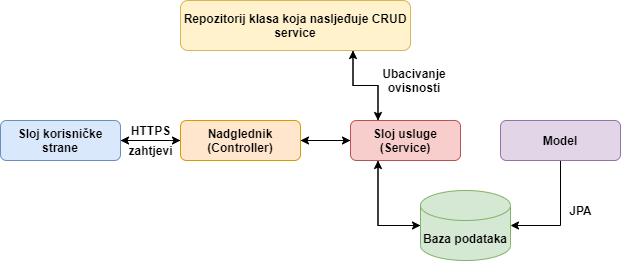
\includegraphics[scale=0.75]{slike/arhitektura.PNG} %veličina slike u odnosu na originalnu datoteku i pozicija slike
	\centering
	\caption{Spring Boot arhitektura}
	\label{fig:spring}
\end{figure}

Želimo li, radi lakšeg razumijevanja, našu arhitekturu usporediti sa stilom MVC (Model-View-Controller), možemo uočiti da se neki slojevi djelomično poklapaju. Primjerice sloj modela kod MVC-a
odgovarao bi sloju domene kod Spring Boota, sloj nadglednika kod MVC-a sloju
nadglednika kod Spring Boota, a sloj pogleda bio bi sloj korisničke strane. 


\vspace{15pt}
Kao što je navedeno, sloj korisničke strane (frontend) je implementiran u Java Scriptu koristeći knjižnicu React. \textbf{React} je besplatna biblioteka otvorenog koda za programski jezik JavaScript koja omogucava razvoj korisničkih sučelja SPA (eng. single-page application). SPA aplikacija je
tip web-aplikacije koja u interakciji s korisnikom dinamički mijenja dijelove stranice, za razliku od tradicionalnih web-aplikacija koje učitavaju cijele nove stranice s poslužitelja. One se pokreću u browseru i ne zahtijevaju ponovno učitavanje nakon korištenja.
React omogućava sastavljanje korisničkog sučelja pomoću elemenata koji se nazivaju komponente. Njih je mogucće iznova koristiti u aplikaciji proizvoljno veliki broj puta. Taj pristup pokazao se lakši za održavanje, proširivanje i višestruko korištenje.

\newpage



	
		

		

				
		\section{Baza podataka}
			
			U sklopu svih zahtjeva vezanih uz razvoj aplikacije nalaze se različiti entiteti i opisi veza među njima. Nijedno se najčešće ne zadaje eksplicitno, već se od inženjera očekuje da ih prepozna, nekako zapiše i pravilno implementira u svoj sustav. Kako bi sve te entitete prikazali na jednom mjestu te kako bi mogli pohranjivati informacije o njima važno je razviti dobru bazu podataka. Baza podataka za koju smo se odlučili u ovome projektu je relacijska; njen glavni objekt je relacija. Jedna relacija predstavlja jedan entitet. Svaka relacija je prikazana u obliku tablice koja ima svoje ime i atribute koji ju opisuju. Tablice su međusobno povezane pri čemu treba pripaziti na vrste veza među njima.  
			Baza podataka se sastoji od 6 glavnih entiteta:
			
			\begin{itemize}
				\item Walker 
				\item Shelter
				\item Walk
				\item Reservation
				\item Dog
				\item Location 
			\end{itemize}
		
			Značenje entiteta i opisi veza među njima su dani ispod. 
			
			\vspace{15pt}
			
			\subsection{Opis tablica}
			
			\vspace{10pt}
			
			\subsubsection{Walker}
			
				Tablica Walker predstavlja registriranog šetača/građana. Nakon što se korisnik aplikacije registrirao u sustavu, ili prijavio ukoliko već ima korisnički račun, on postaje registrirani šetač. Svaki registrirani šetač ima atribute poput imena, prezimena, adrese e-pošte i podataka za prijavu (korisničko ime i lozinka). Taj šetač ima opciju rezervacije termina i psa za šetnju. Iz tog razloga je povezan jedino s entitetom Reservation čija će uloga biti objašnjena ispod. Svaki šetač ima statistiku i raspored svojih šetnji. Ta dva entiteta nisu prepoznata kao zasebne tablice već kao potencijalni upiti nad rezervacijama koje je taj šetač napravio u sustavu. Važan atribut svakog šetača je statVisibility koji označava hoće li se šetačeva statistika šetanja vidjeti na javno dostupnoj rang listi. Svaki šetač ima opciju postavljanja te statistike kao javne ili privatne ovisno o vlastitim preferencijama. 
				
				\filbreak
				
				\begin{longtabu} to \textwidth {|X[6, l]|X[6, l]|X[20, l]|}
					
					\hline \multicolumn{3}{|c|}{\textbf{WALKER}}	 \\[3pt] \hline
					\endfirsthead
					
					\hline \multicolumn{3}{|c|}{\textbf{WALKER}}	 \\[3pt] \hline
					\endhead
					
					
					\hline 
					\endlastfoot
					
					\cellcolor{LightGreen}walkerId & INT	&  	Jedinstveni identifikator šetača 	\\ \hline
					firstName	& VARCHAR &  Ime šetača 	\\ \hline 
					lastName	& VARCHAR &  Prezime šetača 	\\ \hline 
					password & VARCHAR &  Hash lozinka šetača za login u sustav \\ \hline 
					email & VARCHAR &  Adresa e-pošte šetača \\ \hline 
					username & VARCHAR	&  Korisničko ime šetača		\\ \hline 
					statsVisibility	& BOOLEAN &  (Ne)vidljivost šetačeve statistike šetnji javno 	\\ \hline 
						
				\end{longtabu}
			
			\vspace{15pt}
			
			
			\subsubsection{Reservation}
			
				Tablica Reservation predstavlja logičku poveznicu između tri entiteta. Naime, svaki pas kojeg je šetač odabrao za neki termin biva zapisan u zasebnu rezervaciju. Na taj način je omogućeno da se različiti psi nalaze u šetnji kod istog šetača. Svaka rezervacija sadržava 4 atributa, svoj identifikator koji nam u pogledu razumijevanja modela ne znači previše i ostala 3 koja zapravo definiraju jednu rezervaciju.  Ti atributi su: walkId, walkerId i dogId. Zapisi (n-torke) u tablici rezervacija nam daju jasne informacije o tome koji šetači su šetali koje pse i u kojim terminima. Na taj način smo kreirali tablicu iz koje pomoću jednostavnih upita možemo doći do statistika šetnji, kako za pse tako i za šetače.  
			
			
				\begin{longtabu} to \textwidth {|X[6, l]|X[6, l]|X[20, l]|}
		
					\hline \multicolumn{3}{|c|}{\textbf{RESERVATION}}	 \\[3pt] \hline
					\endhead
					
					\hline \multicolumn{3}{|c|}{\textbf{RESERVATION}}	 \\[3pt] \hline
					\endhead
					
					\hline 
					\endlastfoot
					
					\cellcolor{LightGreen}reservationId & INT	&  	Jedinstveni identifikator rezervacije	\\ \hline
					\cellcolor{LightBlue} walkerId	& INT &  Jedinstveni identifikator šetača 	\\ \hline 
					\cellcolor{LightBlue} walkId & INT &  Jedinstveni identifikator šetnje \\ \hline 
					\cellcolor{LightBlue} dogId &INT	&  	Jedinstveni identifikator psa	\\ \hline 
					
				\end{longtabu}
			\newpage
			
			\subsubsection{Walk}
		
				Tablica Walk predstavlja jedan ugovoreni termin šetnje. Budući da je preko entiteta Reservation povezana s psima i šetačima, ne možemo direktno u n-torkama ove tablice vidjeti koji pas je sudjelovao u kojoj šetnji niti dobiti informaciju tko ga je šetao. Ukoliko poznajemo identifikator šetnje i ne koristimo druge tablice možemo saznati dvije informacije, a to su: datum i vrijeme početka i trajanje same šetnje. Kako bi se nova n-torka unijela u ovu tablicu nužno je da šetač napravi rezervaciju čime se implicitno podrazumijeva da se njen termin i ugovoreno trajanje tu zapisuje. 
		
				\begin{longtabu} to \textwidth {|X[6, l]|X[6, l]|X[20, l]|}
				
					\hline \multicolumn{3}{|c|}{\textbf{WALK}}	 \\[3pt] \hline
					\endfirsthead
					
					\hline \multicolumn{3}{|c|}{\textbf{WALK}}	 \\[3pt] \hline
					\endhead
					
					\hline 
					\endlastfoot
					
					\cellcolor{LightGreen}	walkId & INT &  Jedinstveni identifikator šetnje \\ \hline 
					dateTime	&TIMESTAMP &  Datum i vrijeme početka šetnje 	\\ \hline 
					duration & INT &  Duljina šetnje u minutama \\ \hline 
		
				\end{longtabu}
			
			\vspace{5pt}
			
			\subsubsection{Dog}
			
			
				Tablica Dog predstavlja psa. Svaki pas ima udrugu kojoj pripada, s time da je jasno da više pasa može pripadati istoj udruzi. Osim oznake kojoj udruzi pas pripada, on ima atribute koji označavaju njegovu lokaciju, ime, sliku i kratak opis. Osim toga svaki pas ima naznačeno koji tip šetnje preferira (grupne ili individualne). Individualna šetnja pretpostavlja da će jedan registrirani šetač rezervirati samo jednog psa za neki termin te će time napraviti jednu rezervaciju. Grupna šetnja označava situaciju u kojoj šetač odabire više pasa za isti termin te time radi onoliko rezervacija koliko je pasa odabrao. 
	
				\begin{longtabu} to \textwidth {|X[6, l]|X[6, l]|X[20, l]|}
				
					\hline \multicolumn{3}{|c|}{\textbf{DOG}}	 \\[3pt] \hline
					\endfirsthead
					
					\hline \multicolumn{3}{|c|}{\textbf{DOG}}	 \\[3pt] \hline
					\endhead
					
					\hline 
					\endlastfoot
					
					\cellcolor{LightGreen}dogId & INT	&  	Jedinstveni identifikator psa	\\ \hline
					image	& VARCHAR &   URI slike psa	\\ \hline 
					description & VARCHAR &  Opis psa \\ \hline 
					typeOfWalk & VARCHAR	&  	Tip šetnje za koju je pas predodređen (skupna/individualna)	\\ \hline 
					name	& VARCHAR & Ime psa  	\\ \hline 
					\cellcolor{LightBlue} shelterId &  INT	&  	Jedinstveni identifikator udruge	\\ \hline 
					\cellcolor{LightBlue} locationId & INT	&  	Jedinstveni identifikator lokacije	\\ \hline 
					
				
				\end{longtabu}
			
			
			\subsubsection{Shelter}
			
				Tablica Shelter predstavlja udrugu koja se u kontekstu aplikacije smatra drugom vrstom prijavljenog korisnika (osim već spomenutog šetača). Udruga ima svoj profil koji prikazuje slike i kratke opise pasa koji joj pripadaju. Osim informacije s kojim psima udruga raspolaže ona ima i svoje ime, OIB, lokaciju na kojoj se nalazi i naravno podatke za prijavu (korisničko ime i lozinku). Udruga raspolaže statistikom o šetnjama svojih pasa koja se također prikazuje na njenom profilu. Do te statistike se također dolazi putem pregleda svih rezervacija na kojima su njeni psi sudjelovali.   


				\begin{longtabu} to \textwidth {|X[6, l]|X[6, l]|X[20, l]|}
				
					\hline \multicolumn{3}{|c|}{\textbf{SHELTER}}	 \\[3pt] \hline
					\endfirsthead
					
					\hline \multicolumn{3}{|c|}{\textbf{SHELTER}}	 \\[3pt] \hline
					\endhead
					
					\hline 
					\endlastfoot
					
					\cellcolor{LightGreen}	shelterId &  INT	&  	Jedinstveni identifikator udruge	\\ \hline 
					password & VARCHAR &  Hash lozinka šetača za login u sustav \\ \hline 
					name	& VARCHAR &  Ime udruge	\\ \hline 
					username & VARCHAR	&  Korisničko ime udruge	\\ \hline 
					OIB	& VARCHAR &  OIB udruge	\\ \hline 
					\cellcolor{LightBlue} locationId & INT	&  	Jedinstveni identifikator lokacije	\\ \hline 
				
				\end{longtabu}
			
			
			\subsubsection{Location}
			
				Tablica Location predstavlja geografsku lokaciju. Tu lokaciju mogu imati udruge i psi. Pretpostavili smo da se dvije udruge neće nalaziti na istoj lokaciji budući da ju definiraju grad i točna adresa. No, više pasa može živjeti na istoj lokaciji te time ograničenje između broja pasa i lokacije ne postoji. Informacije o lokaciji udruge se nalaze na profilu udruge, dok se lokacija nekog psa vidi u slučaju da ga neki šetač želi rezervirati.
			
				\begin{longtabu} to \textwidth {|X[6, l]|X[6, l]|X[20, l]|}
					
					\hline \multicolumn{3}{|c|}{\textbf{LOCATION}}	 \\[3pt] \hline
					\endfirsthead
					
					\hline \multicolumn{3}{|c|}{\textbf{LOCATION}}	 \\[3pt] \hline
					\endhead
					
					\hline 
					\endlastfoot
					
					\cellcolor{LightGreen}	locationId &  INT	&  	Jedinstveni identifikator lokacije	\\ \hline 
					city & VARCHAR &  Grad \\ \hline 
					adress	& VARCHAR &  Adresa\\ \hline 
					
				\end{longtabu}
			
			
			\subsection{Dijagram baze podataka}
				
				\vspace{15pt} 
				\begin{figure}[H]
					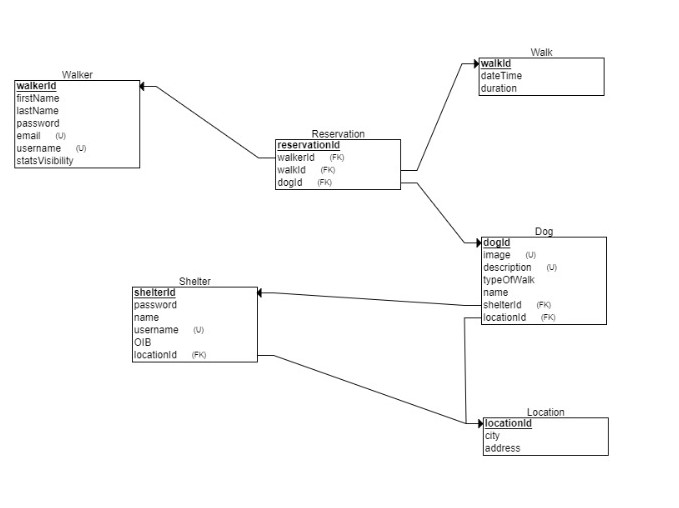
\includegraphics[scale=0.9]{dijagrami/relacijski.jpeg} %veličina slike u odnosu na originalnu datoteku i pozicija slike
					\centering
					\caption{Relacijski dijagram baze podataka}
					\label{fig:relacijski}
				\end{figure}
				\vspace{15pt}
			
			\eject
			
			
		\section{Dijagram razreda}
		
		\iffalse
			\textit{Potrebno je priložiti dijagram razreda s pripadajućim opisom. Zbog preglednosti je moguće dijagram razlomiti na više njih, ali moraju biti grupirani prema sličnim razinama apstrakcije i srodnim funkcionalnostima.}\\
			
			\textbf{\textit{dio 1. revizije}}\\
			
			\textit{Prilikom prve predaje projekta, potrebno je priložiti potpuno razrađen dijagram razreda vezan uz \textbf{generičku funkcionalnost} sustava. Ostale funkcionalnosti trebaju biti idejno razrađene u dijagramu sa sljedećim komponentama: nazivi razreda, nazivi metoda i vrste pristupa metodama (npr. javni, zaštićeni), nazivi atributa razreda, veze i odnosi između razreda.}\\
			
			\fi
			
			
			Na slikama su prikazani dijagrami razreda koji predstavljaju backend dio MVC arhitekture ostvarene korištenjem Java Spring Boota.
			
			\vspace{15pt} 
			\begin{figure}[H]
				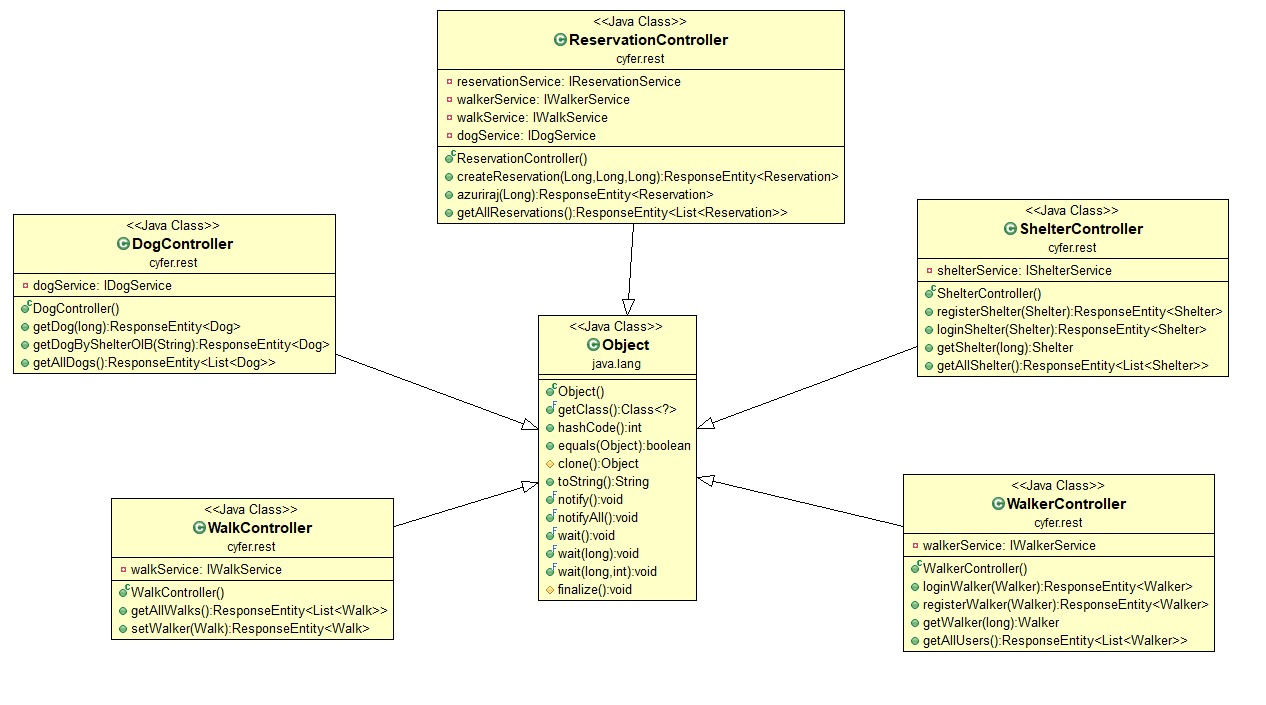
\includegraphics[scale=0.38]{dijagrami/controlleri.jpeg} %veličina slike u odnosu na originalnu datoteku i pozicija slike
				\centering
				\caption{Razredi controlleri}
				\label{fig:controlleri}
			\end{figure}
			
			
			Razredi prikazani na slici ~\ref{fig:controlleri} predstavljaju MVC Kontrolere čije metode mapiraju određene zahtjeve putem URI-a, te vraćaju JSON datoteke koje se potom obrađuju na određeni način. Također šalju i HTML statusni kod.
			Kontroleri su implementirani za pet klasa tipa Model: Dog, Walk, Shelter, Walker i Reservation. Svaki razred ima konstruktor i metode koje mapiraju određene zahtjeve zadanim HTTP zahtjevom.
			
				\vspace{15pt} 
			\begin{figure}[H]
				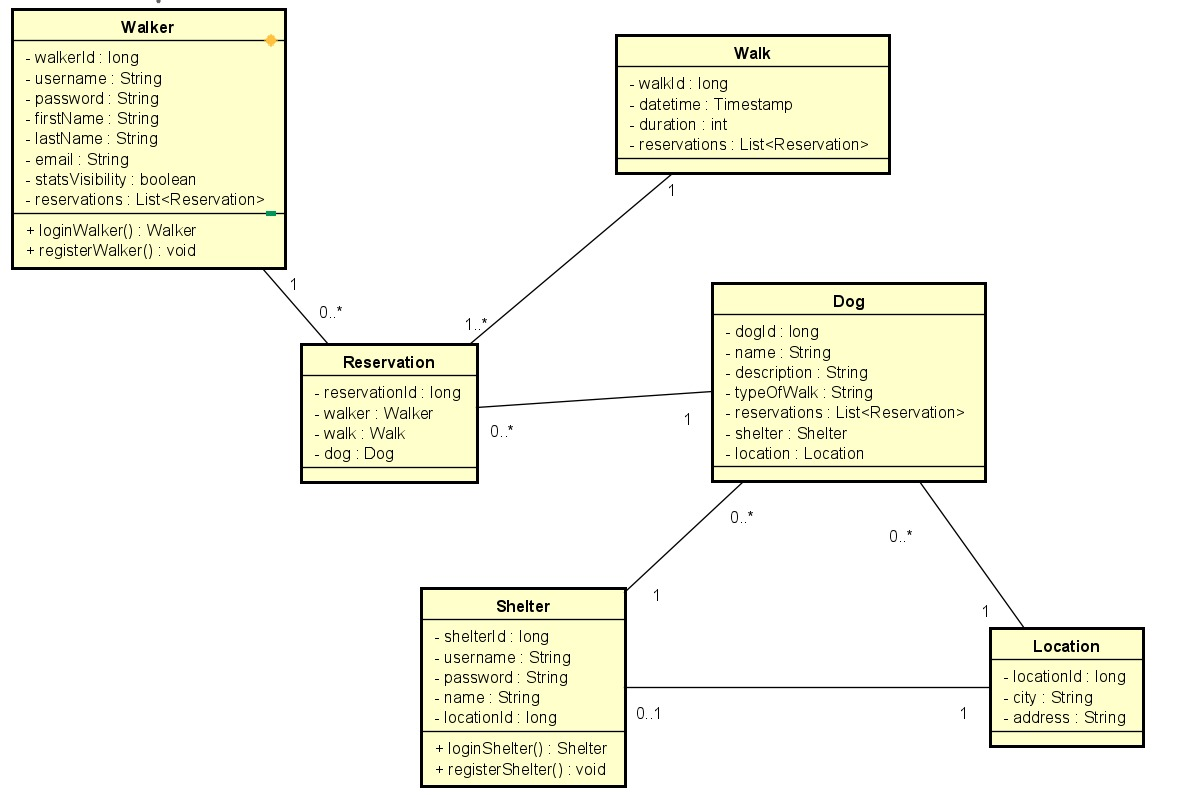
\includegraphics[scale=0.4]{dijagrami/modeli.jpeg} %veličina slike u odnosu na originalnu datoteku i pozicija slike
				\centering
				\caption{Razredi modeli}
				\label{fig:modeli}
			\end{figure}
			
			
		Razredi prikazani na slici ~\ref{fig:modeli} predstavljaju MVC Modele koji odgovaraju entitetima u bazi podataka. Svaki razred sadrži svoj konstruktor, privatne članske varijable koje su mu svojstvene i koje odgovaraju atributima u bazi, kao i sve gettere i settere.
		Razred Dog predstavlja psa koji je pridruženoj određenoj udruzi (Shelter) i dostupan je za šetnje. Razred Walker predstavlja registriranog korisnika (šetača) koji može odabrati psa/pse za šetnju. Razred Shelter predstavlja registriranu udrugu koja ima svoj profil i pse dostupne za šetnju. Razred Walk predstavlja šetnju koja se dogodila s jednim šetačom i jednim ili više pasa. Razred Location predstavlja lokaciju (grad i adresa) na kojoj može biti smješten pas ili udruga. Kardinalnosti veza među razredima su prikazane na dijagramu.
			
			
			\iffalse
			\textbf{\textit{dio 2. revizije}}\\			
			
			\textit{Prilikom druge predaje projekta dijagram razreda i opisi moraju odgovarati stvarnom stanju implementacije}
			
			\fi
			
			\eject
		
		\section{Dijagram stanja}
			
			
			\textbf{\textit{dio 2. revizije}}\\
			
			\textit{Potrebno je priložiti dijagram stanja i opisati ga. Dovoljan je jedan dijagram stanja koji prikazuje \textbf{značajan dio funkcionalnosti} sustava. Na primjer, stanja korisničkog sučelja i tijek korištenja neke ključne funkcionalnosti jesu značajan dio sustava, a registracija i prijava nisu. }
			
			
			\eject 
		
		\section{Dijagram aktivnosti}
			
			\textbf{\textit{dio 2. revizije}}\\
			
			 \textit{Potrebno je priložiti dijagram aktivnosti s pripadajućim opisom. Dijagram aktivnosti treba prikazivati značajan dio sustava.}
			
			\eject
		\section{Dijagram komponenti}
		
			\textbf{\textit{dio 2. revizije}}\\
		
			 \textit{Potrebno je priložiti dijagram komponenti s pripadajućim opisom. Dijagram komponenti treba prikazivati strukturu cijele aplikacije.}